% Copyright 2008 V. Bos, T. van Deursen, and S. Mauw
% This file is part of the MSC Macro Package.
%
\documentclass[12pt,a4paper]{article}
\usepackage{a4wide}
\usepackage{url}
\usepackage{moreverb}
\usepackage{multicol}
\usepackage{msc}
\usepackage{lipsum} 
\usepackage{paralist}
\usepackage{verbatim}
\usepackage{fancyvrb}
\usepackage{relsize}
% \usepackage{adjustbox,lipsum}
\usepackage{array}
\usepackage{listings}
\usepackage{minipage-marginpar}
\usepackage{graphicx}
\usepackage{caption}
\usepackage{subcaption}
\usepackage{subfig}
\usepackage{array}
\usepackage{booktabs}

% we allow a ragged right
\setlength{\rightskip}{0pt plus 0.05\linewidth minus 0pt}
\newlength{\rpwidth}
\setlength{\rpwidth}{.5cm}
\newlength{\rpheight}
\setlength{\rpheight}{0.5\levelheight}
\newcommand{\rpN}{%
  \psframe(-0.5\rpwidth,-\rpheight)(0.5\rpwidth,0\rpheight)%
  \rput[B](0\rpwidth,-0.8\rpheight){\tiny \textsc{n}}%
  \pscircle[fillstyle=solid,fillcolor=black](0\rpwidth,0\rpheight){.5\labeldist}%
}
\newcommand{\rpNE}{%
  \psframe(-\rpwidth,-\rpheight)(0\rpwidth,0\rpheight)%
  \rput[B](-.5\rpwidth,-0.8\rpheight){\tiny \textsc{ne}}%
  \pscircle[fillstyle=solid,fillcolor=black](0\rpwidth,0\rpheight){.5\labeldist}%
}
\newcommand{\rpE}{%
  \psframe(-\rpwidth,-.5\rpheight)(0\rpwidth,.5\rpheight)%
  \rput[B](-.5\rpwidth,-0.3\rpheight){\tiny \textsc{e}}%
  \pscircle[fillstyle=solid,fillcolor=black](0\rpwidth,0\rpheight){.5\labeldist}%
}
\newcommand{\rpSE}{%
  \psframe(-\rpwidth,0\rpheight)(0\rpwidth,\rpheight)%
  \rput[B](-.5\rpwidth,0.2\rpheight){\tiny \textsc{se}}%
  \pscircle[fillstyle=solid,fillcolor=black](0\rpwidth,0\rpheight){.5\labeldist}%
}
\newcommand{\rpS}{%
  \psframe(-.5\rpwidth,\rpheight)(.5\rpwidth,0\rpheight)%
  \rput[t](0\rpwidth,0.8\rpheight){\tiny \textsc{s}}%
  \pscircle[fillstyle=solid,fillcolor=black](0\rpwidth,0\rpheight){.5\labeldist}%
}
\newcommand{\rpSW}{%
  \psframe(0\rpwidth,0\rpheight)(\rpwidth,\rpheight)%
  \rput[B](.5\rpwidth,0.2\rpheight){\tiny \textsc{sw}}%
  \pscircle[fillstyle=solid,fillcolor=black](0\rpwidth,0\rpheight){.5\labeldist}%
}
\newcommand{\rpW}{%
  \psframe(0\rpwidth,-.5\rpheight)(\rpwidth,.5\rpheight)%
  \rput[B](.5\rpwidth,-0.3\rpheight){\tiny \textsc{w}}%
  \pscircle[fillstyle=solid,fillcolor=black](0\rpwidth,0\rpheight){.5\labeldist}%
}
\newcommand{\rpNW}{%
  \psframe(0\rpwidth,-\rpheight)(\rpwidth,0\rpheight)%
  \rput[B](.5\rpwidth,-0.8\rpheight){\tiny \textsc{nw}}%
  \pscircle[fillstyle=solid,fillcolor=black](0\rpwidth,0\rpheight){.5\labeldist}%
}

% The following code is taken from the doc package. It defines a global 
% macro \bslash that produces a bslash (if present in the current font). 
\makeatletter
{\catcode`\|=\z@ \catcode`\\=12 |gdef|bslash{\}}
\makeatother
\newcommand{\cmd}[1]{\texttt{\bslash #1}}

\newcommand{\acro}[1]{{#1}}

\newcommand{\MSC}{\acro{MSC}}
\newcommand{\HMSC}{\acro{HMSC}}
\newcommand{\MSCdoc}{\MSC{}doc}
\newcommand{\mscpack}{\MSC{} macro package}

\newcommand{\env}[1]{\texttt{#1}}
\newcommand{\opt}[1]{[#1]}
\newcommand{\cmdarg}[1]{\{\emph{#1}\}}
\newcommand{\coordarg}[1]{\emph{#1}}
\newcommand{\coordargs}[2]{(\coordarg{#1},\coordarg{#2})}
\newcommand{\lnsvalue}[3]{large/normal/small value #1/#2/#3}

\newenvironment{defs}{%
  \begin{list}{}%
              {\setlength{\labelwidth}{0pt}%
               \setlength{\labelsep}{1em}%
               \setlength{\leftmargin}{1em}%
               \setlength{\parsep}{1ex}%
               \setlength{\listparindent}{0pt}%
               \setlength{\rightmargin}{0pt}%
               \renewcommand{\makelabel}[1]{##1}%
               \raggedright%
              }%
  }{%
  \end{list}}


\title{
  VULFI: An Instruction-level Fault Injection Framework\\{\large User Manual}
}

\author{
 \begin{tabular}{c}
  \begin{tabular}{cc}
   Vishal Sharma &
   Ganesh Gopalakrishan  \\
   %
    \multicolumn{2}{c}{\scriptsize School of Computing, University of Utah} \\
   %
   \multicolumn{2}{c}{\scriptsize \texttt{\{vcsharma,ganesh\}@cs.utah.edu}} \\
  \end{tabular}\\
 \end{tabular}
}

\date{\small Version 1.0, last updated \today\\
%       Describing \mscpack{} version \mscversion
      }

\begin{document}


\maketitle

\newpage

\tableofcontents

\newpage

\section{Getting Started}
\label{started}
VULFI is an instruction-level fault injection framework which is developed using LLVM compiler infrastructure\cite{lattner2004,llvmwebref}.
%
VULFI targets LLVM's intermediate representation (IR) level instructions for fault injections.
%
VULFI is capable of targeting vector instructions (including architecture specific intrinsics) in addition to scalar instructions
for fault injections.
%
Visit VULFI's home page (\url{http://formalverification.cs.utah.edu/fmr/vulfi/}) and fill out the request form to obtain a copy 
of VULFI.

\section{Requirements}
\label{prereq}

\subsection{Supported Languages}
\label{lang}
VULFI is capable of targeting any high-level program which can be compiled into LLVM IR. Currently, VULFI has been extensively tested 
with C, C++, and ISPC programs.

\subsection{Software Requirements}
\label{softreq}
\begin{compactitem}
\item \textbf{OS} : Ubuntu 12.04 LTS.

 \item \textbf{LLVM} : VULFI has been developed using LLVM version 3.2. LLVM documentation:\\ \url{http://llvm.org/releases/3.2/docs/GettingStarted.html#getting-started}.
 
 \item \textbf{ISPC}: In case you are targeting ISPC programs for the fault injection, please use ISPC 
 version 1.8.1 (download link: \url{http://sourceforge.net/projects/ispcmirror/files/}) 
 
 \item \textbf{Python}: Install Python version 2.7 or later.
 
 \item \textbf{OpenCV} (optional) : Install OpenCV version 2.3.1. Installation steps: \\
 \url{http://www.samontab.com/web/2012/06/installing-opencv-2-4-1-ubuntu-12-04-lts/}.
\end{compactitem}


% 
% \section{Code Documentation}
% \label{docu}
% VULFI's code documentation is maintained at: \url{http://formalverification.cs.utah.edu/fmr/vulfi/doc/}.

\section{License \& Copyright Information}
\label{license}
Before using VULFI, please refer to the \texttt{LICENSE} file located in the topmost directory of the 
distribution. 
%
Please note that the VULFI distribution contains 3rd party programs which may have different license 
and copyright requirements than VULFI.
%
You must always adhere to the individual license and copyright requirements of the 3rd party 
programs in addition to the VULFI license and copyright requirements.
%
%
The license and copyright information for the 3rd party programs is provided in the \texttt{LICENSE} file.

% \subsection{VULFI License}
% \label{vulfi-license}
% 
% \subsection{ISPC License}
% \label{ispc-license}
% 
% \subsection{ISPC Benchmark License}
% \label{ispc-bench-license}
% 
% \subsection{PARVEC Benchmark License}
% \label{parvec-license}

% \subsection{SCL Benchmark License}
% \label{scl-license}

\section{Installation}
\label{install}

\begin{enumerate}
 \item Change directory to the LLVM lib directory and copy VULFI source code to 
 the current directory.
 \begin{Verbatim}[fontsize=\relsize{-1},frame=single,framerule=0.1mm]
 $ cd [LLVM_SRC_ROOT_DIR]/lib/ 
 \end{Verbatim} 
 
 \item Change directory to the VULFI lib directory.
 \begin{Verbatim}[fontsize=\relsize{-1},frame=single,framerule=0.1mm]
 $ cd vulfi/lib 
 \end{Verbatim}
 
 \item Run below commands to install a shared library (\texttt{relief.so}) containing VULFI implementation .
 \begin{Verbatim}[fontsize=\relsize{-1},frame=single,framerule=0.1mm]
  $ make 
  $ sudo make install 
 \end{Verbatim}  
\end{enumerate}

% \caption{An example C++ function \texttt{foo()}}
% \label{fig:foo}
% \vspace{-0.5cm}
% \end{figure}

% \subsection{OpenCV Installation}
% \label{opencv-install}
% 
% \subsection{VULFI Installation}
% \label{vulfi-install}

\section{Usage}
\label{usage}
Performing fault injection using VULFI is a two-step process.
%
First, we instrument a target program using VULFI.
%
This step involves compiling the target program into an LLVM
bitcode file.
%
The target bitcode file is then linked with the VULFI's \texttt{Corrupt.bc}
bitcode file containing callable runtime fault injection APIs. 
%
The resultant bitcode is then instrumented using the VULFI LLVM pass.
%
Second, we execute the resultant instrumented binary using python script
for performing fault injection.
%
The automation script provides a rich set of command line options
to effectively analyze the result of a fault injection run, and for generating a
detailed fault injection report. 


\subsection{Step 1: Instrumenting a Target Program for Fault Injection}
Given that VULFI is implemented as an LLVM pass, a target program bitcode
is instrumented by running VULFI on it with \texttt{opt}
(\url{http://llvm.org/docs/WritingAnLLVMPass.html#running-a-pass-with-opt}).
Below are the command line options supported by VULFI:

\begin{Verbatim}[fontsize=\relsize{-1},frame=single,framerule=0.1mm,commandchars=\\\{\}]
 -fn                                 Name of the functions (separated by a single 
                                     white space) to be targeted for fault injections.
                                     Example: -fn "foo1 foo2 foo3"
             
 -fsa \{data,dint,dflo,ctrl,addr\}     Fault site selection algorithm; valid options:
                                     data: Target all pure-data fault sites for fault 
                                     injection. Specifically, target all fault sites 
                                     with its: (1) Lvalues of Integer or FloatingPoint 
                                     types, and (2) forward program slice of the 
                                     fault sites does contain an instruction 
                                     with Lvalue of Pointer or Control type.
                                     
                                     dint: Same as "data" option except that target 
                                     fault sites of only Integer types.
                                     
                                     dflo: Same as "data" option except that target 
                                     fault sites of only FloatingPoint types.
                                     
                                     Note:- For Integer type, the supported 
                                     bit-widths are 8, 16, 32, and 64. For 
                                     FloatingPoint type, the supported 
                                     formats are single (32-bit) and double 
                                     precision (64-bit) floating-point values.
                                  
                                     
                                     ctrl: Target all fault sites of Integer or 
                                     FloatingPoint type such that its forward program 
                                     slice must contain atleast one contol instruction 
                                     (e.g., "cmp" instruction).
                                     
                                     addr: Target all fault sites which either
                                     have its Lvalue of Pointer type or its
                                     forward program slice must contain atleast one 
                                     instruction of Pointer type.
                                     (e.g., "getElementPtr" instruction).

 -rf \{0,1\}                           Range flag used to indicate if fault injection 
                                     has to be done in a specific code section (using 
                                     the source code line numbers). It is disabled 
                                     (set to 0) by deafult.
 
 -flr                                Name of the csv file containing range information. 
                                     This is an optional argument used only when -rf 
                                     is enabled. 
 
 -lang \{C,C++,ISPC\}                  The language option is used by VULFI to check for 
                                     language specific information which may be useful 
                                     for fault injection. For example, language 
                                     specific metadata information.
 
 -arch \{x86,neon,nvvm,mips,spu\}      This architecture information is used when 
                                     instrumenting architecture specific intrinsics 
                                     for fault injection. This includes information 
                                     such as whether an intrinsic uses mask. Currently, 
                                     x86 is the only supported architecture; other 
                                     architectures are just a placeholder and may
                                     be supported in future. 
 
 -dbgf                               Name of the CSV file to which the list of static 
                                     fault sites (instrumented for runtime fault 
                                     injection) is written.
\end{Verbatim}


\subsection{An Example Instrumentation}
For a target C++ program file \texttt{foo.cpp}
having function definitions \texttt{foo()}
and \texttt{main()}, the first mandatory step is to 
add following function prototypes at the beginning of the file:
%
%
\begin{Verbatim}[fontsize=\relsize{-1},frame=single,framerule=0.1mm]
extern int printFaultSitesData(void);
extern int printFaultInjectionData(void); 
\end{Verbatim}
%
%
Next, add the below functions calls in the function \texttt{main()}
just before every return statements.
\begin{Verbatim}[fontsize=\relsize{-1},frame=single,framerule=0.1mm]
printFaultSitesData();
printFaultInjectionData(); 
\end{Verbatim}
%
%
%
The modified C++ program file \texttt{foo.cpp} is then
compiled into a bitcode \texttt{foo.bc} as shown below:
%
\begin{Verbatim}[fontsize=\relsize{-1},frame=single,framerule=0.1mm]
 $ clang++ -emit-llvm foo.cpp -c -o foo.bc
 \end{Verbatim}
%
%
Similarly, the program file \texttt{Corrupt.C} located in the
directory \texttt{runtime/}, is compiled into a bitcode \texttt{Corrupt.bc}. 
When using clang++ to compile the Corrupt.C file, add a macro definition
"\_\_CLANGPP" as described below. However, you must not use this macro when
using clang to compile the Corrupt.C file.

%
\begin{Verbatim}[fontsize=\relsize{-1},frame=single,framerule=0.1mm]
$ clang++ -emit-llvm -D__CLANGPP Corrupt.C -c -o Corrupt.bc
\end{Verbatim}
 %
 %
Next, both the bitcode files are linked using \texttt{llvm-link}:
%
\begin{Verbatim}[fontsize=\relsize{-1},frame=single,framerule=0.1mm]
$ llvm-link Corrupt.bc foo.bc -o foo-corrupt.bc
\end{Verbatim}
%
The resultant bitcode file is then instrumented by running VULFI pass 
using \texttt{opt} as shown below:
%
\begin{Verbatim}[fontsize=\relsize{-1},frame=single,framerule=0.1mm]
$ opt -load /usr/local/lib/relief.so -vulfi  -fn "foo" -fsa "data" -lang "C++"
-dbgf "instruction_list_foo.csv" < foo-corrupt.bc > foo-inject.bc
\end{Verbatim}
%
%
Finally, the instrumented and the uninstrumented binaries (\texttt{foo-inject} and \texttt{foo} 
respectively) are generated.
%
%
\begin{Verbatim}[fontsize=\relsize{-1},frame=single,framerule=0.1mm]
$ clang++  foo-inject.bc -o foo-inject

$ clang++  foo.bc -o foo
\end{Verbatim}
%
Both the binaries are executed under a given program input. 
%
The execution output of \texttt{foo-inject} is compared with that of
\texttt{foo} to detect the occurrence of a silent data corruption in
the former execution output.
%

\subsection{Step 2: Automating Fault Injection using Python Script}
\label{cmdopt}

A binary instrumented using VULFI reads fault site selection and 
fault injection related information from a configuration file.
%
The python script \texttt{driver.py} (located at \texttt{vulfi/scripts/})
automates the creation of the configuration file, running the instrumented
binary, and generating the fault injection report.
%
Therefore, we must always using the python script \texttt{driver.py} for 
fault injection runs.
%
The command line options supported by the python script are listed
below:

 \begin{Verbatim}[fontsize=\relsize{-1},frame=single,framerule=0.1mm,commandchars=\\\{\}]
Usage: python driver.py [-h] [-e] [-s] [-c] [--ov] [--pv] [--iter EXEC_COUNT]
                 [--fcp {bex,img,num}] [--th TH] [--exec1 EXEC1] [--cmd1 CMD1]
                 [--out1 OUT1] [--cho] [--cfs] [--exec2 EXEC2] [--cmd2 CMD2]
                 [--out2 OUT2] [--rslt RSLT] [--ficsv FICSV] [--fia {cbr,abr}]
                 [--fib {1,2,3,4,5,6,7,8}] [--fid {msb,lsb}] [--fbu FBU]
                 [--fbl FBL] [--np NUM_PROB] [--dp DEN_PROB]
                 [--ff {eql,max,min,nlm}] [--fc FICOUNT]

Descriptions of the arguments:
-h, --help                Shows this help message and exits.

-e                        Execution mode.

-s                        Standalone mode, always used in combination with 
                          -e option.
                                     
-c                        Comparison mode, always used in combination with 
                          -e option.

--exec1 EXEC1             Location of the 1st executable, EXEC1, to be 
                          executed with -s or -c mode.
                           
--cmd1 CMD1               Command line args (if any) for the exe EXEC1.
                          
--out1 OUT1               Name (including complete path) of the output file 
                          generated by EXEC1.                    

--exec2 EXEC2             Location of the instrumented executable, EXEC2, 
                          to be executed only with -c.
                          
--cmd2 CMD2               Command line args (if any) for the exe EXEC2.
					  
--out2 OUT2               Name (including complete path) of the output file 
                          generated by EXEC2.
                          
--ov                      Calculate overhead.

--pv                      Override user provided fault injection probability 
                          and perform fault injection using a fault injection 
                          probability of 1/N where N is the total number of 
                          dynamic instructions.

--iter EXEC_COUNT         Number of iterations.

--fcp \{bex,img,num\}       Method used for comparing outputs of a fault-free 
                          execution and a fault execution. Valid options for 
                          comparing the outputs:
                          1. bex = Compare and match the outputs bit by bit.
                          2. img = If the outputs are image files, perform 
                          PSNR based comparison.
                          3. num = If the outputs are of numeric type then 
                          express the difference between the outputs
                          as L2Norm.

--th TH                   Threshold value; only valid with --fcp=img or num.
                          Report SDC if the difference in the outputs calculated 
                          using "img" or "num" based method exceeds the threshold TH.
                          
--cho                     This performance flag indicates that use cached output 
                          for exec1 if available. This is disabled by default.
                          WARNING: Enable this option ONLY if you are sure that the 
                          execution output of exec1 is expected to be the same 
                          during every execution iteration.
                          
--cfs                     This performance flag indicates that use cached fault 
                          site count. Use it only when --cho flag is enabled.

--rslt RSLT               Name of the output file where result will be written.

--ficsv FICSV             Name of the input csv file where fault injection report
                           information will be written.

--fia \{cbr,abr\}            Fault injection algorithm, valid options: 
                           1. cbr - cumulative byte ordering; target one or more 
                           contiguous bytes for fault injection.
                           2. abr - absolute bit range;target a bit-range for fault 
                           injection.
                        	
--fib \{1,2,3,4,5,6,7,8\}    Number of contiguous bytes to be considered for fault 
                           injection.
                           Note: this option must be provided when using -fia=cbr

--fid \{msb,lsb\}            Direction from which no. of contiguous bytes to be
                           considered for fault injection.
                           Note:this option must be provided when using -fia=cbr.
                           
--fbu FBU                  Upper bound for the fault injection bit-range.
                           Note:this option must be provided when using -fia=abr.

--fbl FBL                  Lower bound for the fault injection bit-range.
                           Note:this option must be provided when using -fia=abr.
                           
--np NUM_PROB              Numerator of fault injection probability expressed as a
                           fraction.

--dp DEN_PROB              Denominator of fault injection probability expressed as
                           a fraction.
                           
--ff\{eql,max,min,nlm\}      Puts restriction on the fault injection count; 
                           valid options:
                           1. eql - continue injecting faults until fault injection 
                           count becomes equal to the value passed using --fc.
                           2. max - continue injecting faults until fault injection 
                           count is less than or equal to the value passed using 
                           --fc.
                           3. nlm - inject faults in all eligible fault sites.

--fc FICOUNT               Fault injection countm this value is used in combination 
                           with --ff.
 \end{Verbatim}  
 
%  \subsection{An Example of Fault Injection Run using Python Script}

%   \subsection{Fault Injection Algorithm}
%  \label{fia}
%  \subsubsection{Absolute Bit Range (ABR)}
%  \subsubsection{Cumulative Byte Range (CBR)}
 
 
\section{Examples}
\label{examples}
\subsection{Example 1 : Scalar Benchmark - Quicksort }
\label{ex1-qsort}

\subsubsection{Step 1: Compile}
\begin{enumerate}
%
%
\item Change the directory to the source folder:
 \begin{Verbatim}[fontsize=\relsize{-1},frame=single,framerule=0.1mm]
 $ cd vulfi/benchmarks/scalar_benchmarks/src
 \end{Verbatim}
 %
 %
 \item Make sure that the paths provided in \texttt{common.mk} file
 are correct. 
 %
 %
 \item Change directory to qsort folder and compile the program:
 \begin{Verbatim}[fontsize=\relsize{-1},frame=single,framerule=0.1mm]
 $ cd qsort/
 $ cd make
 \end{Verbatim}
 %
 %
 \end{enumerate}

\subsubsection{Step 2: Run}
\begin{enumerate}
 \item Change the directory to the run folder:
 \begin{Verbatim}[fontsize=\relsize{-1},frame=single,framerule=0.1mm]
 $ cd vulfi/benchmarks/scalar_benchmarks/run
 \end{Verbatim}
 %
 %
 \item Make sure that the paths provided in \texttt{common.mk} file
 are correct. 
 %
 %
 \item Change the directory to the qsort folder. The \texttt{common\_qsort.mk} file
 contains the python command line used for performing the fault injection.
 The script file \texttt{run\_qsort.sh} launches the execution accepting
 a single argument to denote the number of fault injection runs to 
 be carried out.
 
 \begin{Verbatim}[fontsize=\relsize{-1},frame=single,framerule=0.1mm]
 $ cd qsort/
 $ ./run_qsort.sh 100
 \end{Verbatim}
 \end{enumerate}
 
 \subsubsection{Step 3: Result Analysis}

 \begin{enumerate}
  \item \textbf{Fault Sites:} Refer to the files \texttt{addr\_dbgData\_qsort\_addr.csv} and \\
  \texttt{ctrl\_dbgData\_qsort\_ctrl.csv} located at \texttt{\textbackslash{vulfi}\textbackslash{benchmarks}\textbackslash{scalar\_benchmarks}
  \textbackslash{src}\textbackslash{qsort}}. These files list the fault sites chosen for runtime fault injection 
  for \texttt{address} and \texttt{control} fault site categories respectively. You may notice that there are no \texttt{data} fault 
  sites found for the qsort program.
  
  \item \textbf{Fault Injection Result:} The fault injection result for each fault site category is saved in the directory
  \texttt{\textbackslash{vulfi}\textbackslash{benchmarks}\textbackslash{scalar\_benchmarks}\textbackslash{run}\textbackslash{qsort}\textbackslash{serial}}.
  For example, each row in the file \texttt{result\_qsort\_ctrl.csv} correspond to a unique fault injection run during which a fault was injected.
  The result file provides useful information such as instruction and bit position chosen at runtime for the fault injection. It also categorizes 
  the result of the fault injection into one of the categories - \texttt{sdc, benign, crash,}  and \texttt{error}.
  
 \end{enumerate}

\subsection{Example 2 : ISPC Benchmark - Raytracing }
\label{ex2-rt}

The steps to run \texttt{Raytracing} benchmark is similar to the previous example. However, this benchmark requires
the ISPC compiler\cite{ispc12,ispcwebref}
to be present on the machine.
%
%
A precompiled version of the ISPC compiler which is known to work with the current version of VULFI could be downloaded from:
\url{https://www.dropbox.com/s/5qjilxsqho14ell/ispc.tar.gz?dl=0}.
%
%
Please make sure that you follow the license requirement of the ISPC compiler (\url{https://ispc.github.io/})
before downloading the precompiled binaries.
%
%

\subsubsection{Step 1: Compile}
\begin{Verbatim}[fontsize=\relsize{-1},frame=single,framerule=0.1mm]
 $ cd vulfi/benchmarks/ispc_benchmarks/src/rt/
 $ make
 \end{Verbatim}
 
\subsubsection{Step 2: Run}
 \begin{Verbatim}[fontsize=\relsize{-1},frame=single,framerule=0.1mm]
 $ cd vulfi/benchmarks/ispc_benchmarks/run/rt/
 $ ./run_rt.sh 5
 \end{Verbatim}
 
\subsubsection{Step 3: Result Analysis}
Figures~\ref{fig:original} and~\ref{fig:corrupted} are the outputs 
generated by the \texttt{Raytracing} benchmark for a fault-free
and a faulty runs respectively.

\begin{enumerate}
 \item \textbf{Files listing fault sites: }
 \begin{Verbatim}[fontsize=\relsize{-1},frame=single,framerule=0.1mm]
addr_dbgData_rt_avx2.csv
addr_dbgData_rt_sse4.csv
addr_dbgData_rt_ser.csv
ctrl_dbgData_rt_avx2.csv
ctrl_dbgData_rt_sse4.csv
ctrl_dbgData_rt_ser.csv
data_dbgData_rt_avx2.csv
data_dbgData_rt_sse4.csv
data_dbgData_rt_ser.csv
 \end{Verbatim}
 \item \textbf{Files with the fault injection results: }
 \begin{Verbatim}[fontsize=\relsize{-1},frame=single,framerule=0.1mm]
result_rt_avx2_addr.csv
 result_rt_sse4_addr.csv
 result_rt_ser_addr.csv
 result_rt_avx2_ctrl.csv
 result_rt_sse4_ctrl.csv
 result_rt_ser_ctrl.csv
 result_rt_avx2_data.csv
 result_rt_sse4_data.csv
 result_rt_ser_data.csv
 \end{Verbatim}
 
\end{enumerate}

\begin{figure}
  \begin{minipage}{0.45\textwidth}
  \centerline{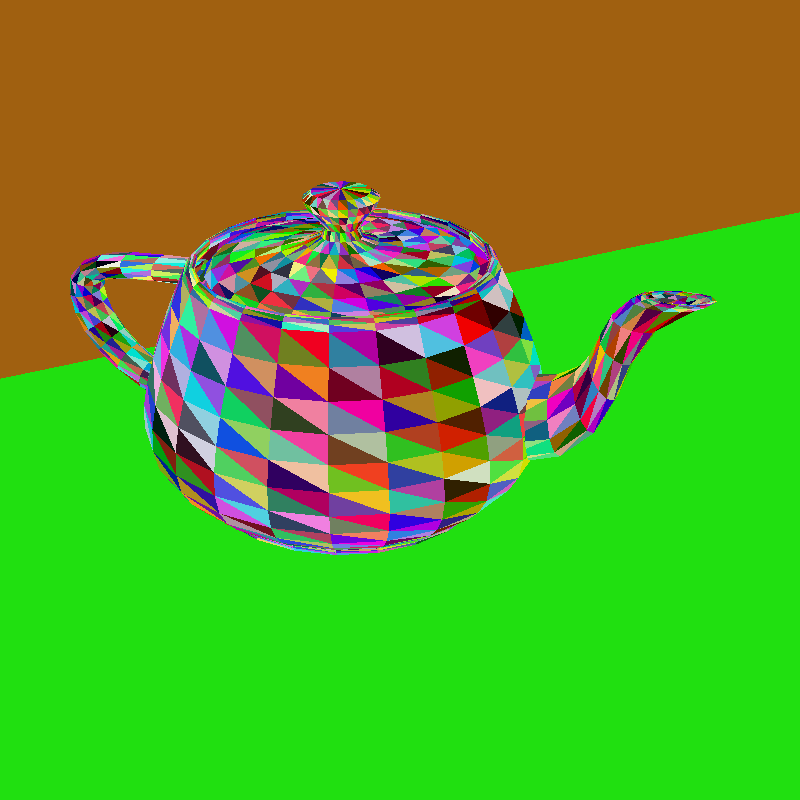
\includegraphics[width=7.2cm,height=6.2cm]{image/teapot.png}}
  \caption{Golden Image}
  \label{fig:original}
  \end{minipage}
  \begin{minipage}{0.45\textwidth}
  \centerline{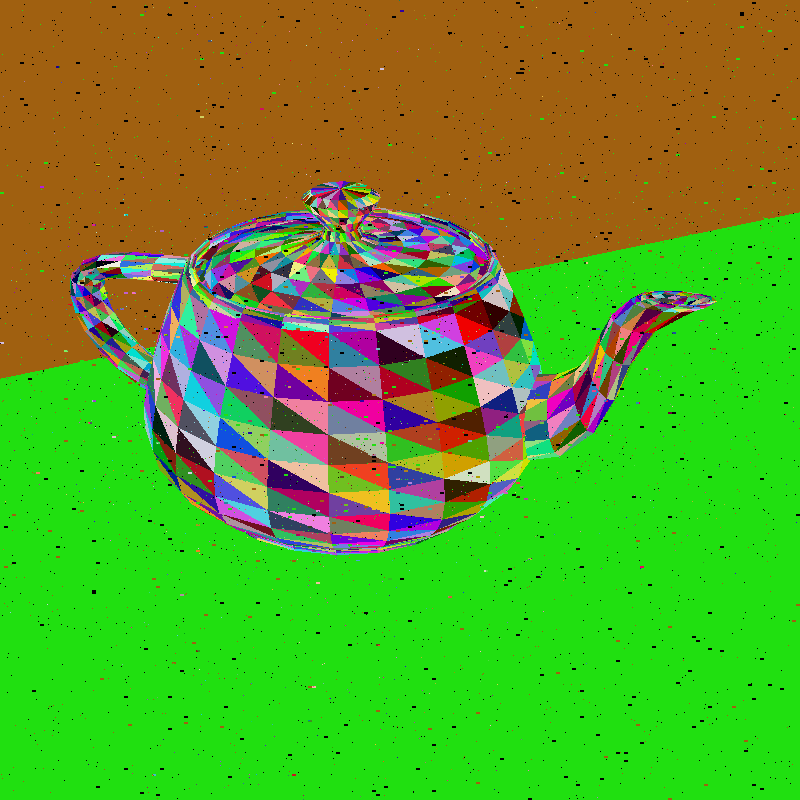
\includegraphics[width=7.2cm,height=6.2cm]{image/teapot-corrupt_fip_1_1000.png}}
  \caption{Corrupted Image}
  \label{fig:corrupted}
  \end{minipage} 
\end{figure}
  
% \section{Extending VULFI}
% \label{extend}
% 
% \subsection{The \texttt{SiteSelector} Class}
% \label{siteselector}
% 
% \subsection{The \texttt{FaultInjector} Class}
% \label{faultinjector}
% 
% \subsection{Runtime Library file \texttt{Corrupt.C}}
% \label{corruptlib}
% 
% \subsection{Updating Intrinsic definitions}
% \label{intdef}


\bibliographystyle{plain}
\bibliography{biblio}

\end{document}
